\providecommand{\main}{../..}
\documentclass[\main/dresen_thesis.tex]{subfiles}
\renewcommand{\thisPath}{\main/chapters/looselyPackedNS}
\begin{document}
  \chapter{Loosely-packed nanostructures}\label{ch:looselyPackedNS}

    \subfile{\thisPath/nanoparticles/nanoparticles}

    \section{Preparation of Loosely-Packed Layers}
      \begin{figure}[tb]
        \centering
        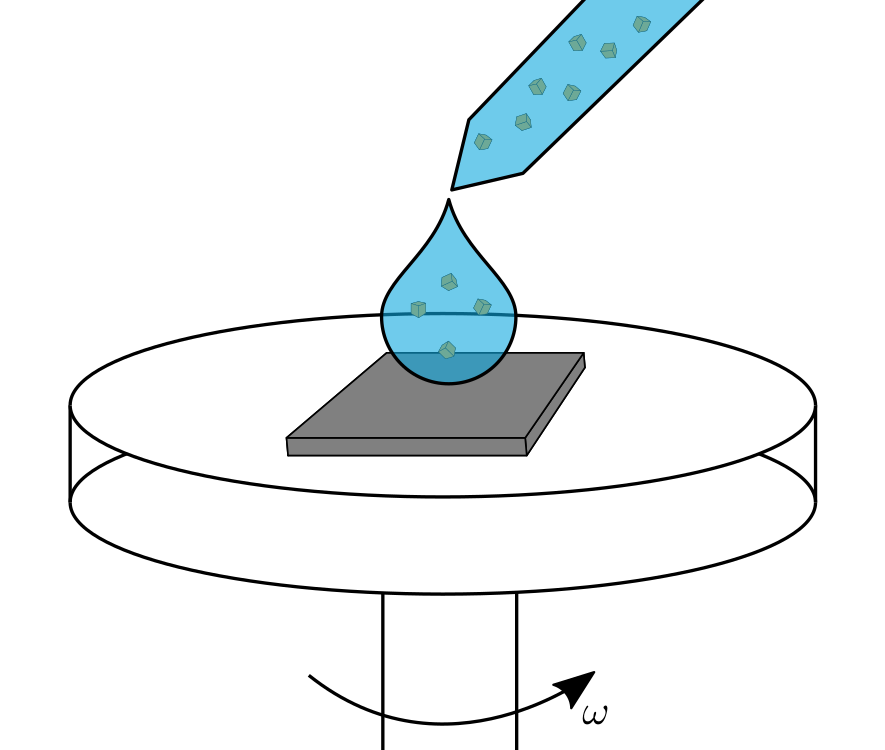
\includegraphics{looselyPackedNP_spinCoatingScheme}
        \caption{\label{fig:looselyPackedNP:preparation:spinCoatingScheme}During spin coating a drop of dispersion is transferred on a substrate, which subsequently is rotated to remove the liquid by centrifugal force leaving behind a thin film of the nanoparticle material.}
      \end{figure}

      A quick and effective way to transfer nanoparticles from a dispersion to a thin layer on a substrate is spin coating.
      Here a droplet of a dispersion with a high concentration of nanoparticles is transferred on a substrate, which subsequently rotates the substrate with a high angular frequency.
      Due to the centrifugal force, most parts of the dispersion is removed from the substrate and only a homogeneous thin layer remains on the substrate.
      The thickness of the thin nanoparticle layer can be tuned by variation of the rotation speed, the nanoparticle concentration in dispersion, and the time that the substrate is rotated.
      On the one hand spin coating produces quickly and effectively thin layers with homogeneous thickness, but on the other hand it is highly inefficient in material usage, as most parts are lost during the process.
      As will be shown in the following, the quick process also has the downside that the nanoparticles generally do not have enough time to self assemble in highly ordered structures.

      Thin layer samples of the previously discussed nanoparticles were prepared by the same collaboration that produced the nanoparticles.
      As substrate, silicon wafers were chosen and pretreated for 30 minutes in a fresh Piranha solution (\ch{H2SO4} [conc.] and \ch{H2O2} [30\%] in a ratio of 2:1). Subsequently they washed with \ch{EtOH} and heated in an oven to $450 ^\circ \mathrm{C}$ for one hour.
      After that procedures any organic remain is removed from the silicon and the nanoparticle dispersion is spin coated on the substrate.

    \section{Nuclear Structure}
      \begin{figure}[tb]
        \centering
        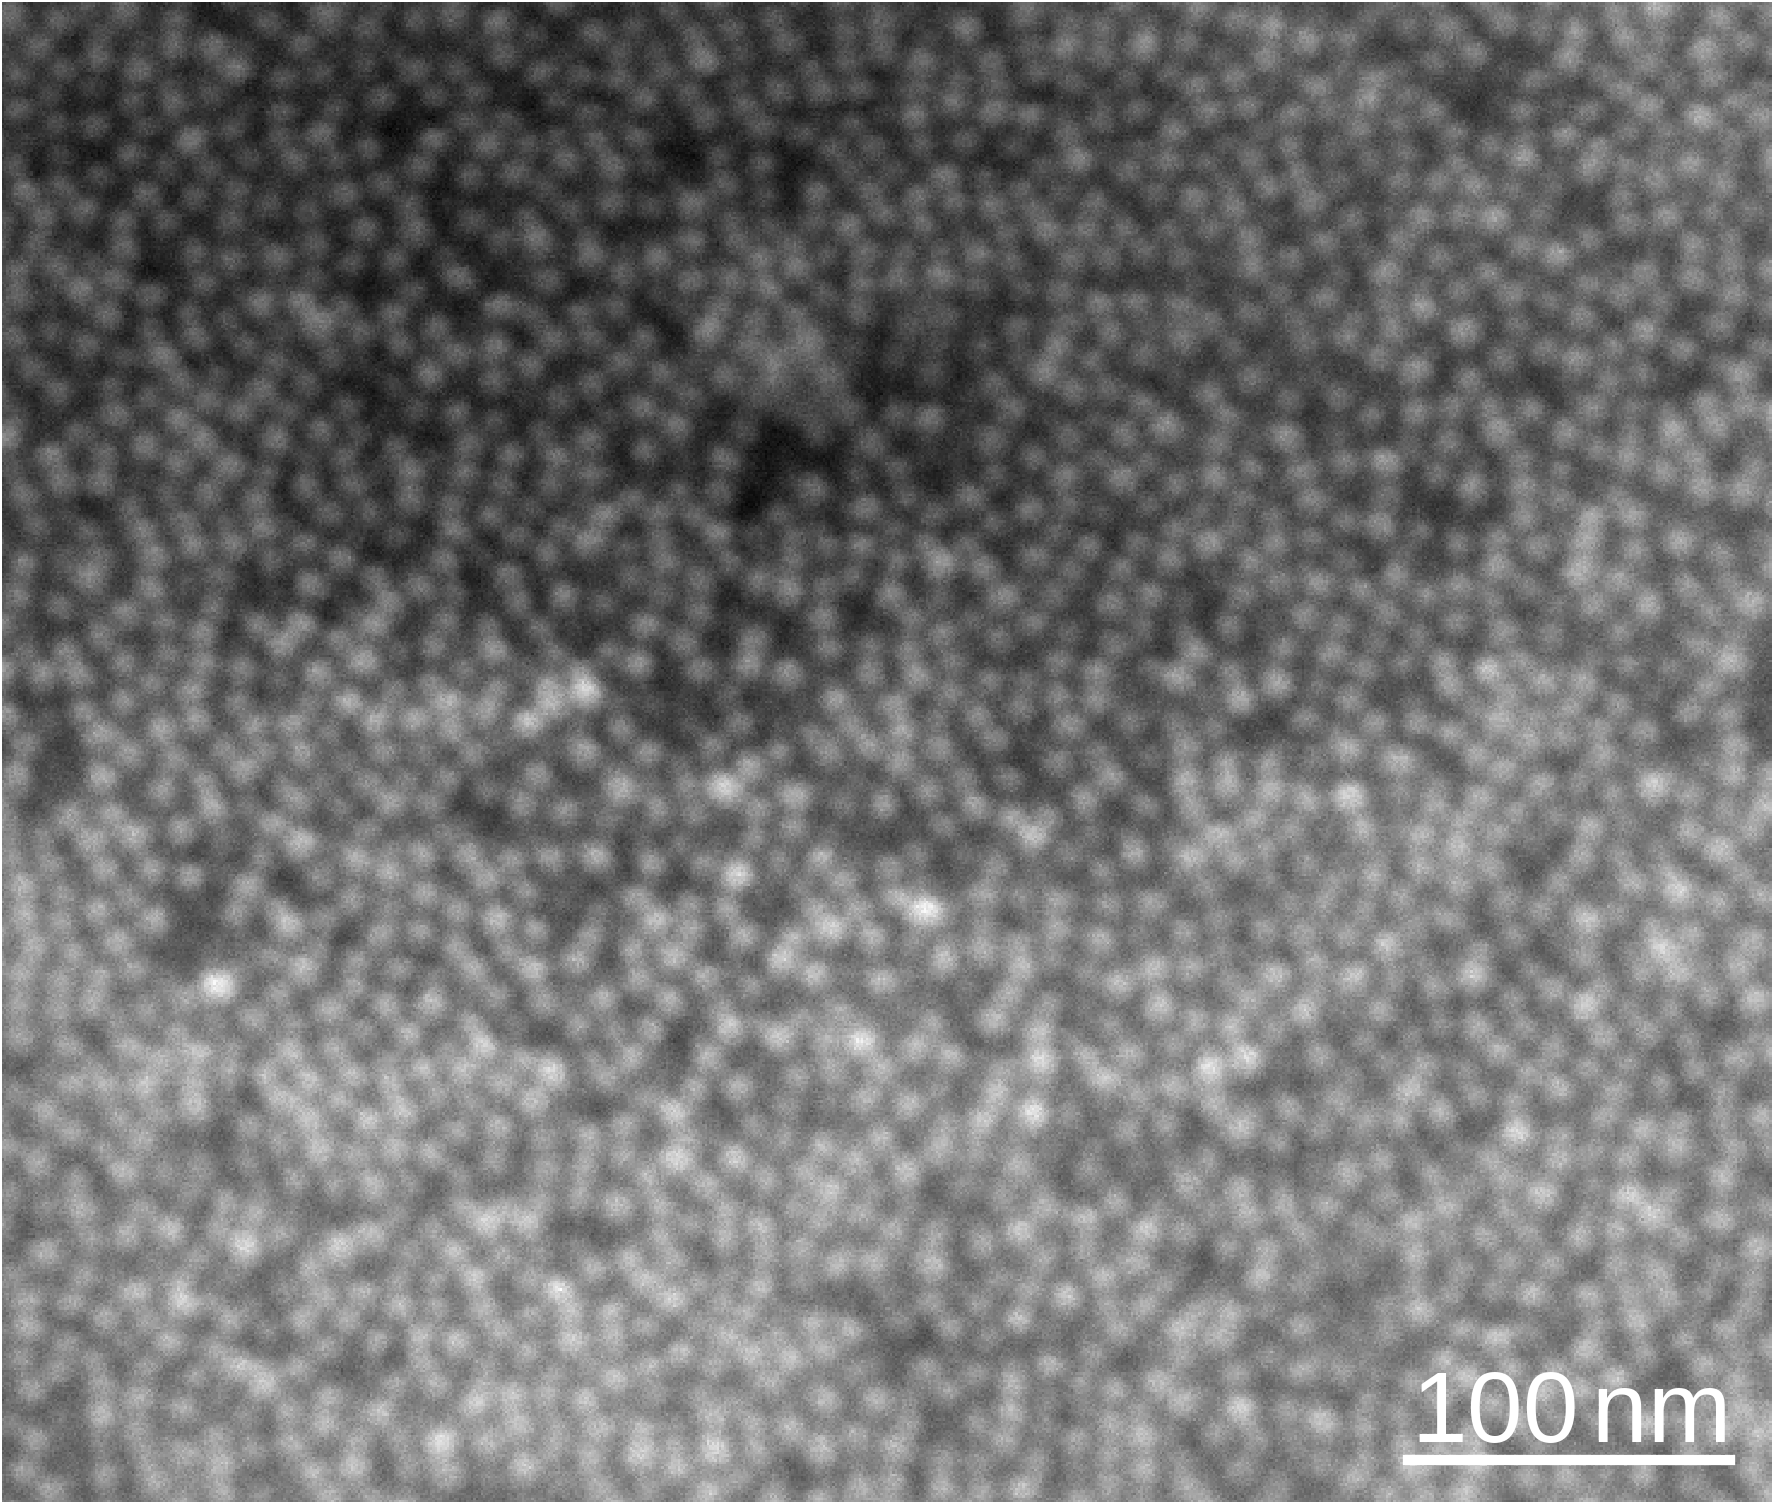
\includegraphics{looselyPackedNP_SEM_ES_S14_TopView}
        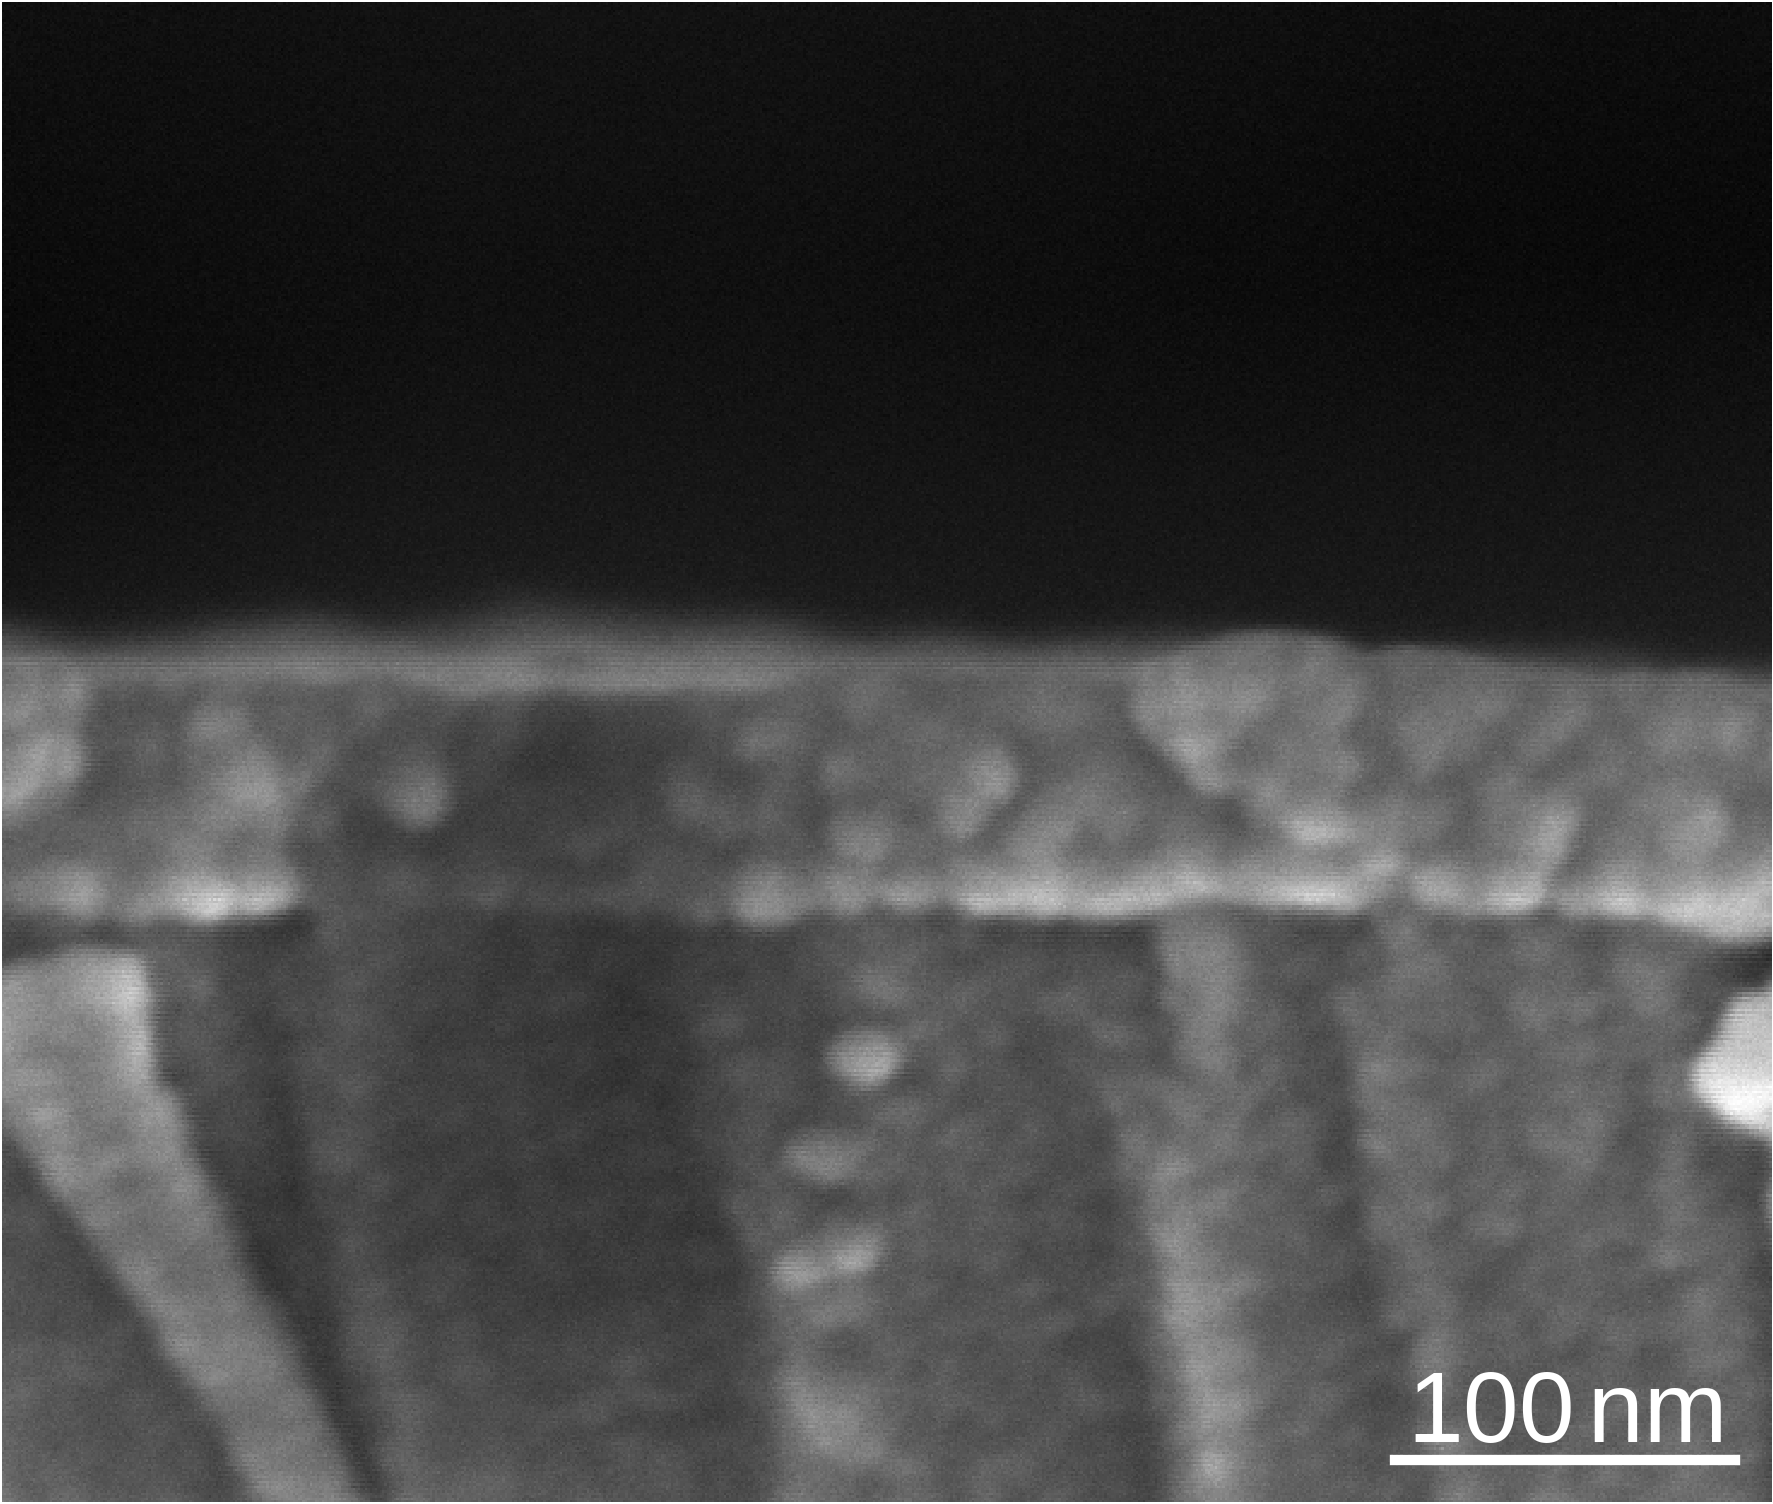
\includegraphics{looselyPackedNP_SEM_ES_S14}
        \caption{\label{fig:looselyPackedNP:nuclearStructure:sem}Scanning electron microscopy view of IOS-11 after spin coating on silicon from the top (left) and in cross section (right).}
      \end{figure}
      In a first step the spin-coated samples are studied structurally.
      By scanning electron microscopy (SEM), images of of the sample are taken at high magnification as shown in \reffig{fig:looselyPackedNP:nuclearStructure:sem}.
      The wafer was carefully broken into two pieces along a straight line to additionally study the cross sectional structure.
      On first glance, the homogeneous flat surface of the sample is visible in the cross section.
      In \reffig{fig:looselyPackedNP:nuclearStructure:semProjection}, the cross section is integrated along the vertical axis to estimate the average height of the sample at this local spot to $\approx 90 \unit{nm}$.

      The top view in \reffig{fig:looselyPackedNP:nuclearStructure:sem} shows no long range order among the nanoparticles and suggests that no dense packing is achieved through spin coating.
      Spheres that do not undergo any ordering process and are packed randomly have been studied extensively on the macroscopic scale \cite{Torquato_2000_IsRan} and it has been shown experimentally that the densest random close packing (RCP) lies in the order of $\approx 64 \, \%$.
      In a long range ordered crystalline structure, the closest packing spheres can achieve are the face-centered cubic and the hexagonal close-packed structure, which have a packing of $74 \, \%$.
      To study the packing of the nanoparticles, x-ray and neutron scattering provide non-destructive tools to quantify the order of the volume fraction across a large area of the sample.
      X-ray and neutron reflectometry is used to study the vertical structure of the sample, and grazing incidence small-angle x-ray scattering to study the lateral structure.

      \begin{figure}[tb]
        \centering
        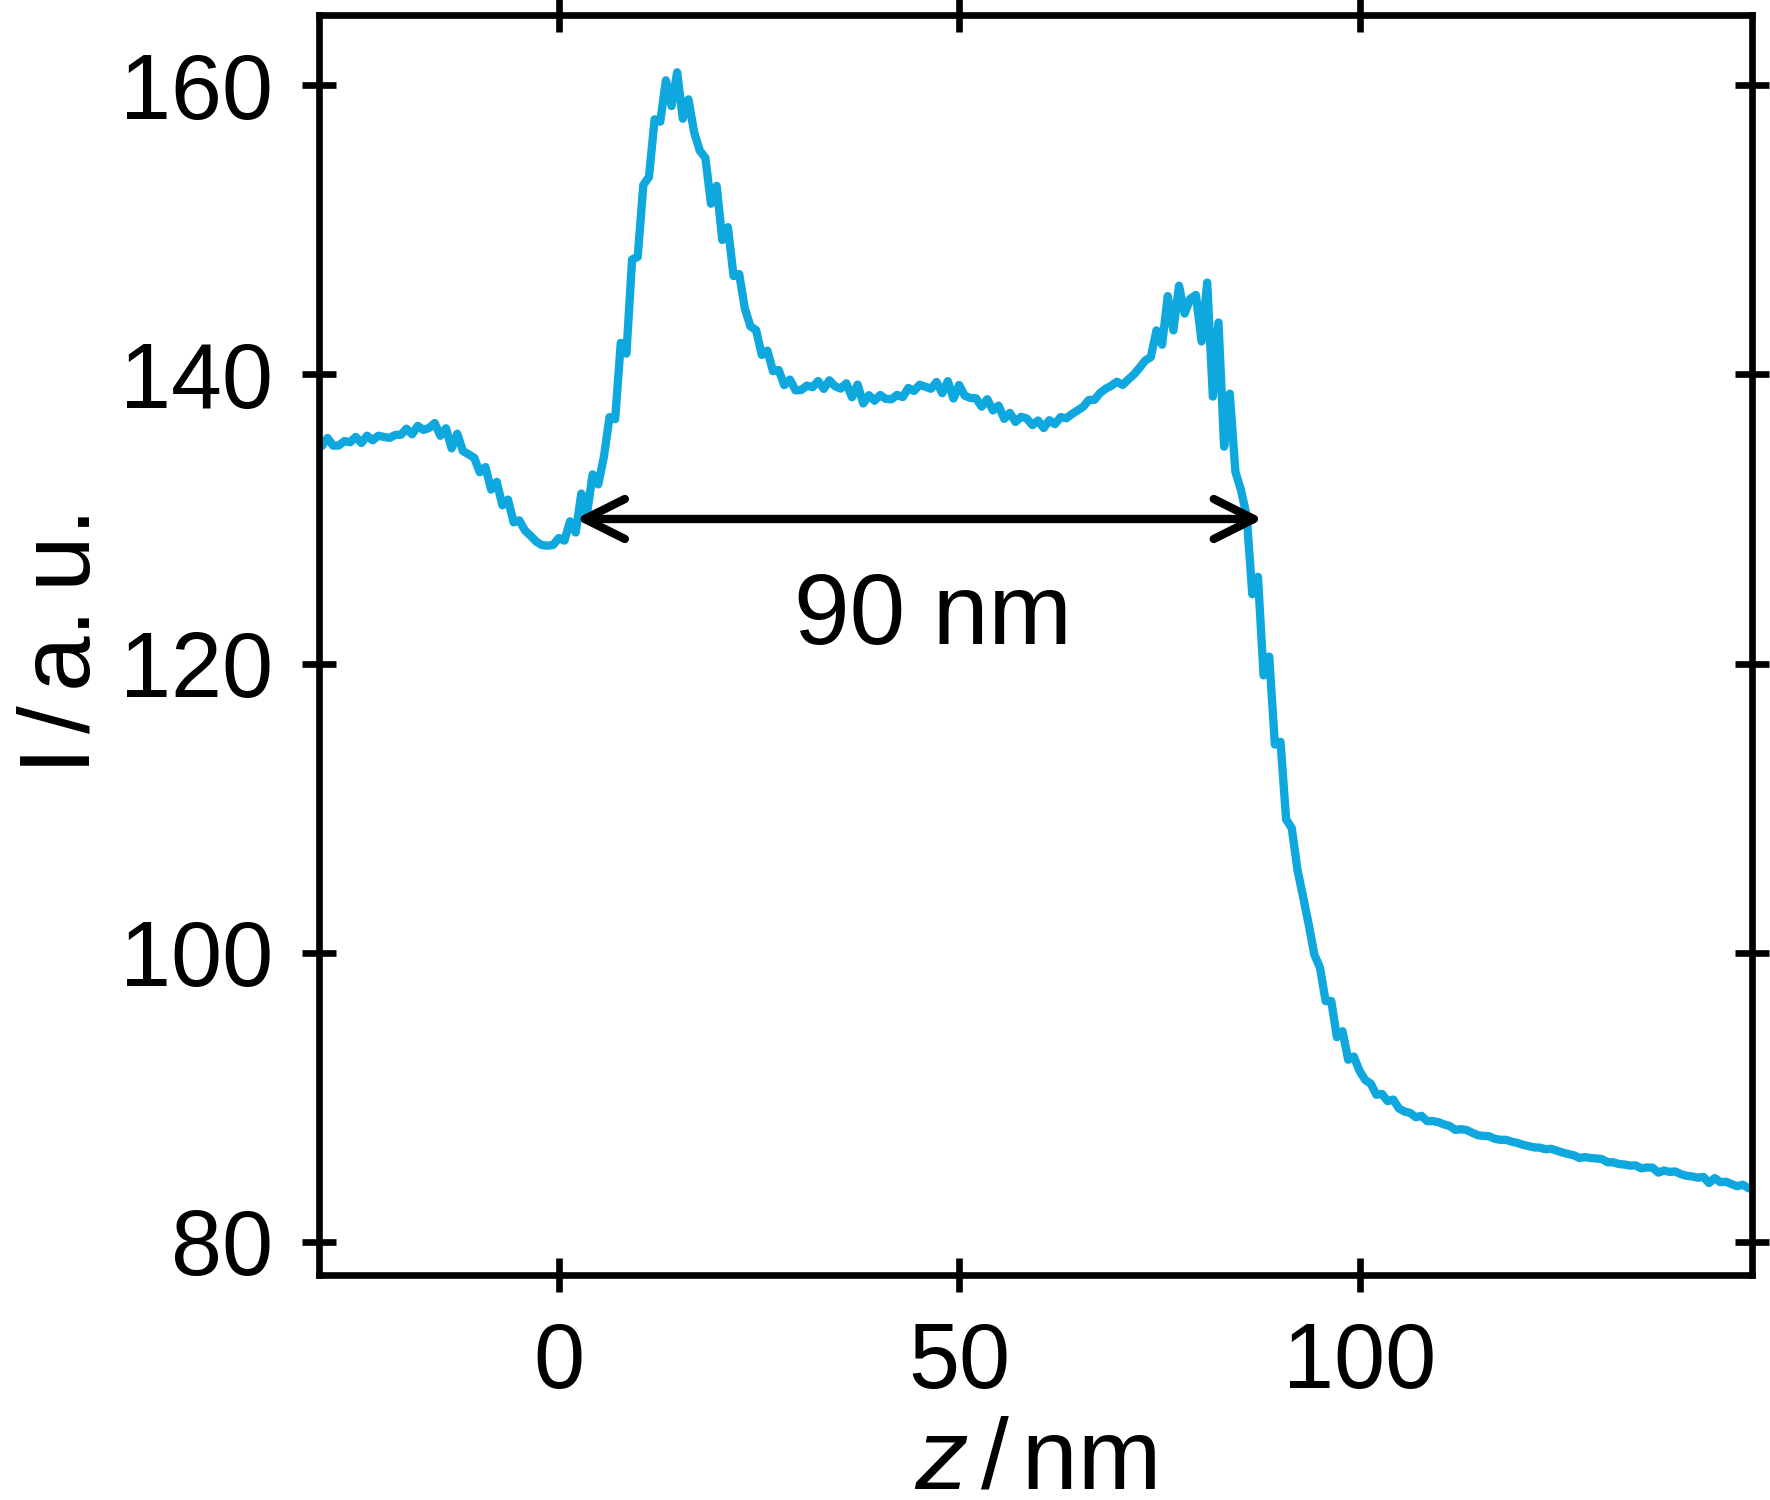
\includegraphics{looselyPackedNP_SEMprojection_ES_S14}
        \caption{\label{fig:looselyPackedNP:nuclearStructure:semProjection}Projection of the pixel intensity along the vertical axis from the cross sectional SEM shown in \reffig{fig:looselyPackedNP:nuclearStructure:sem}.}
      \end{figure}

      \begin{figure}[tb]
        \centering
        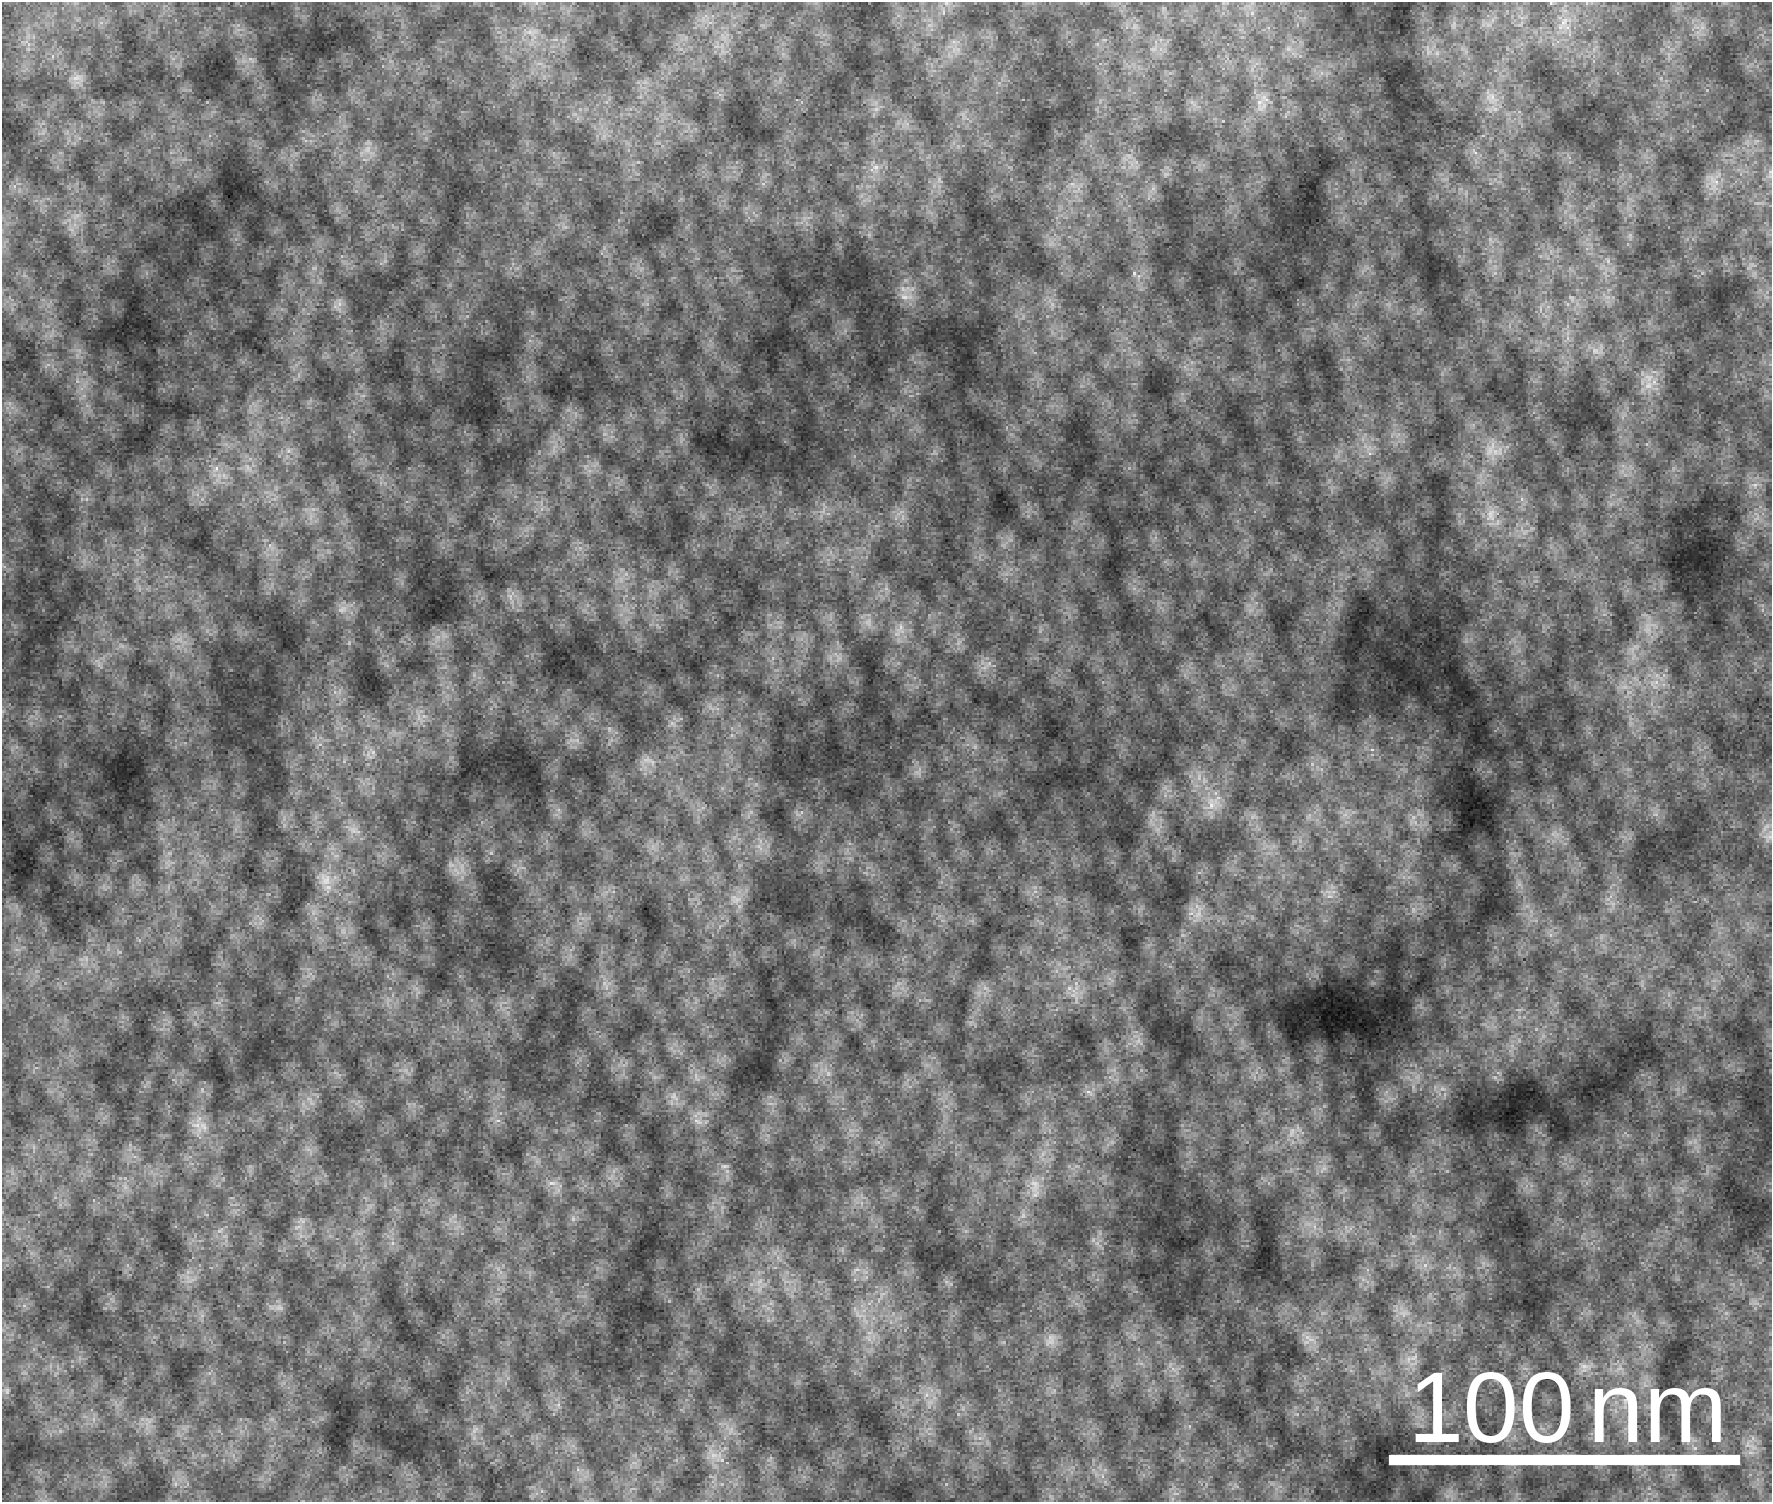
\includegraphics{looselyPackedNP_SEM_ES_S17_TopView}
        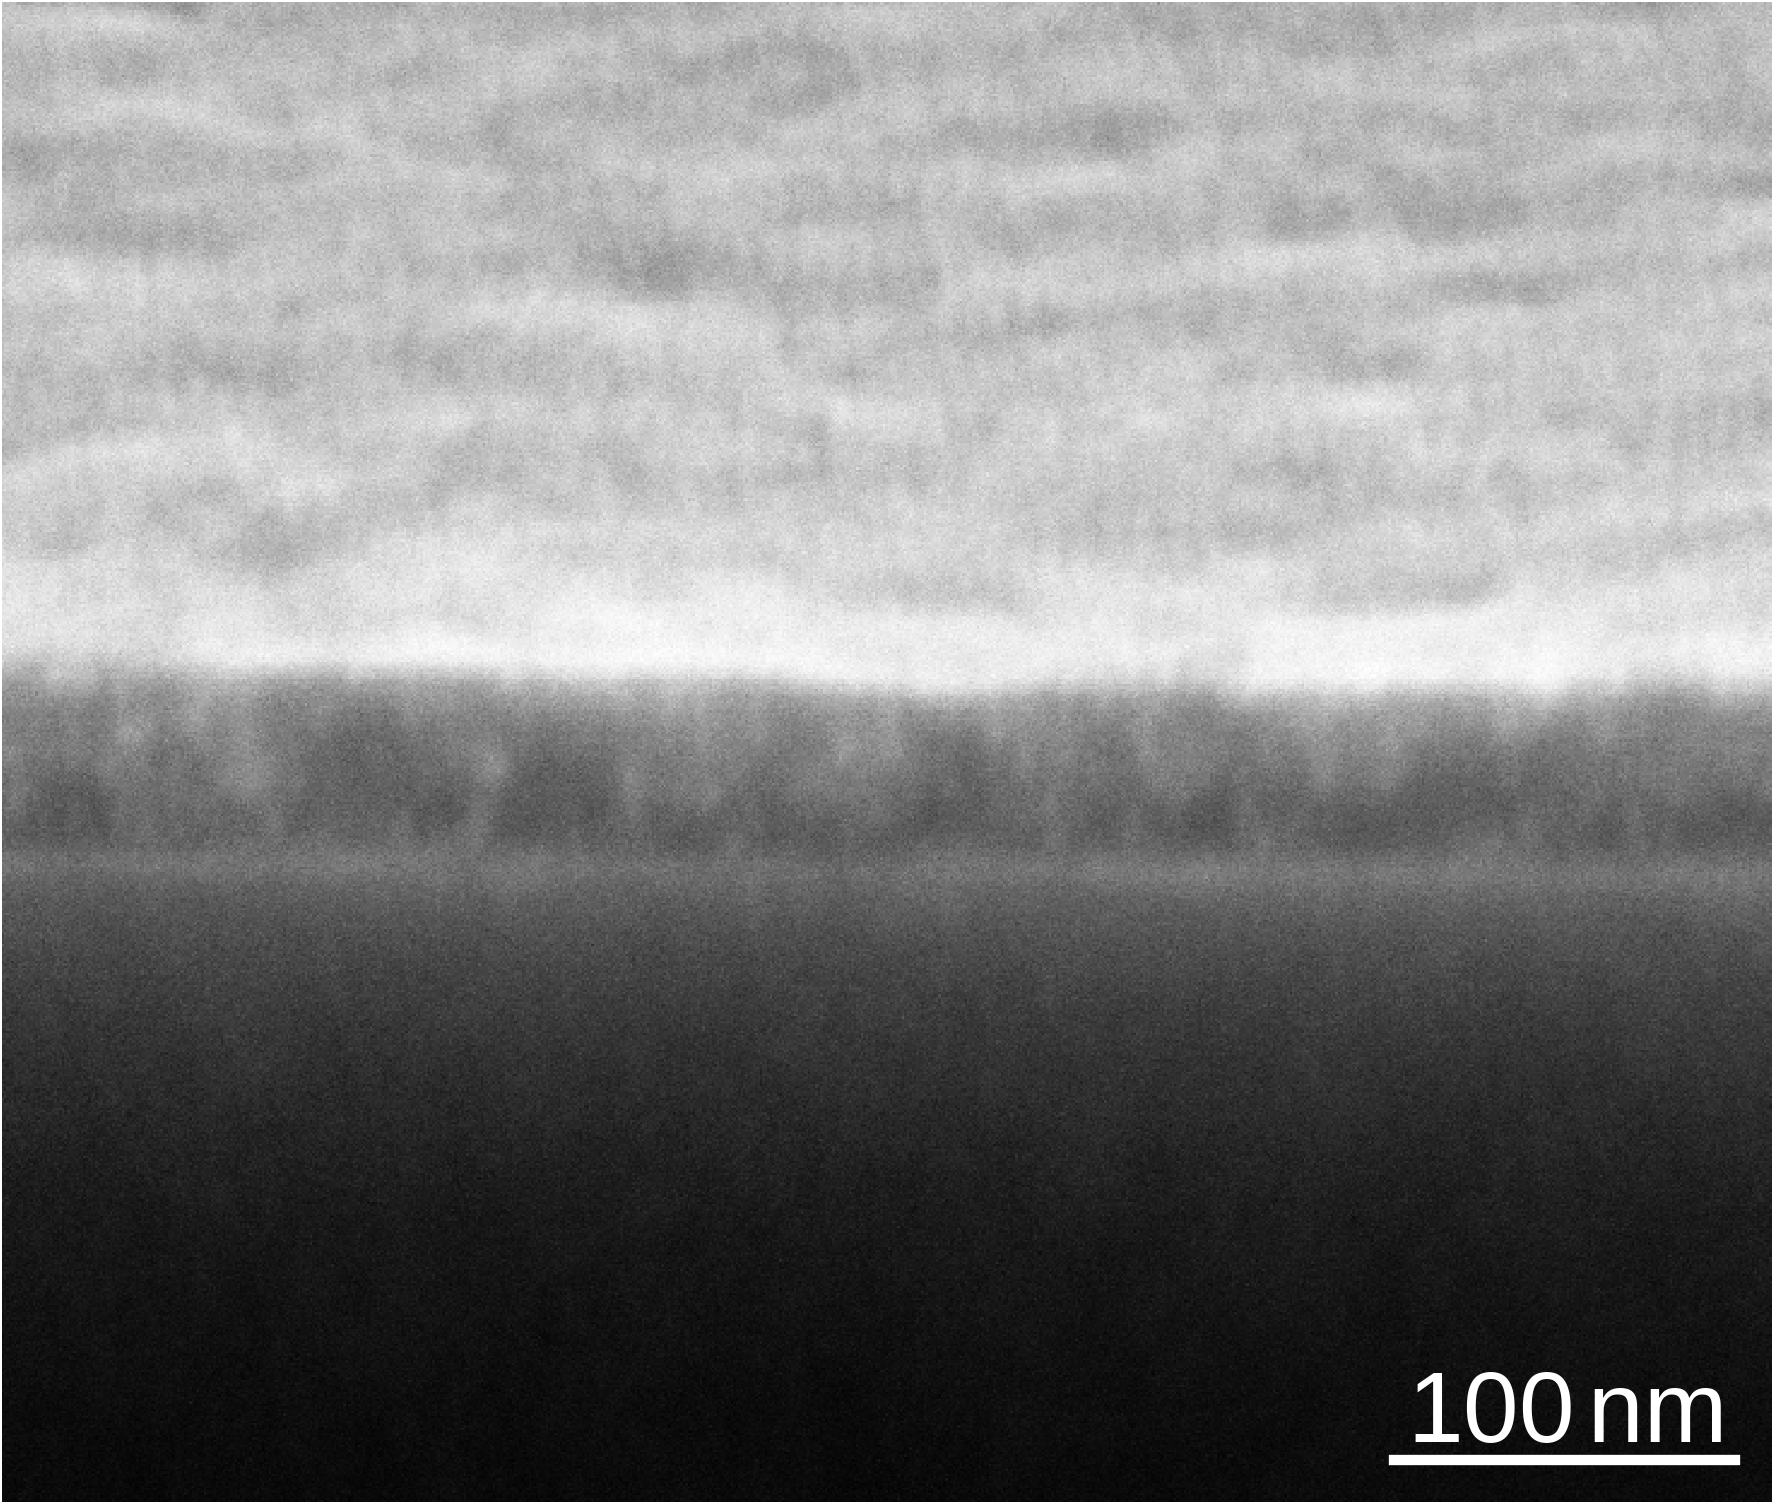
\includegraphics{looselyPackedNP_SEM_ES_S17}
        \caption{\label{fig:looselyPackedNP:nuclearStructure:sem}Scanning electron microscopy view of IOS-7 from the top (left) and in cross section (right).}
      \end{figure}

    \section{Magnetic Structure}

    \section{Emergent Effects}

    \section{Model}

\end{document}